\documentclass[aspectratio=169,11pt]{beamer}
\usepackage[T1]{fontenc}
\usepackage{lmodern,amsmath,amssymb,mathtools,bm,booktabs,array,graphicx,tikz}
\usetikzlibrary{arrows.meta,positioning,calc,decorations.pathreplacing,patterns}
\definecolor{ink}{HTML}{17344D}\definecolor{accent}{HTML}{087E8B}\definecolor{pale}{HTML}{EDF5F5}\definecolor{gold}{HTML}{AD6B19}
\providecommand{\dd}{\,\mathrm{d}}\providecommand{\R}{\mathbb{R}}
\providecommand{\E}{\mathbb{E}}\providecommand{\Var}{\operatorname{Var}}
\providecommand{\Cov}{\operatorname{Cov}}\providecommand{\diag}{\operatorname{diag}}
\providecommand{\norm}[1]{\left\lVert#1\right\rVert}
\providecommand{\abs}[1]{\left|#1\right|}
\usefonttheme{professionalfonts}
\setbeamercolor{normal text}{fg=black,bg=white}
\setbeamercolor{frametitle}{fg=ink,bg=white}
\setbeamercolor{title}{fg=ink}\setbeamercolor{structure}{fg=accent}
\setbeamercolor{block title}{fg=ink,bg=pale}\setbeamercolor{block body}{fg=black,bg=pale!40}
\setbeamercolor{alerted text}{fg=accent}
\setbeamerfont{frametitle}{size=\Large,series=\bfseries}
\setbeamerfont{title}{size=\LARGE,series=\bfseries}
\setbeamertemplate{navigation symbols}{}
\setbeamersize{text margin left=.7cm,text margin right=.7cm}
\setbeamertemplate{frametitle}{\vspace{.18cm}\insertframetitle\par\vspace{.1cm}{\color{accent}\hrule height .6pt}\vspace{.12cm}}
\newcommand{\notestarget}{notes.pdf}\newcommand{\noteslabel}{Notes}
\setbeamertemplate{footline}{\hspace{.7cm}\color{ink}\scriptsize Mathematical Modeling\quad\href{\notestarget}{\noteslabel}\hfill\insertframenumber\,/\,\inserttotalframenumber\hspace{.7cm}\vspace{.18cm}}
\setbeamercovered{invisible}
\hypersetup{pdfauthor={Zan Ahmad},pdftitle={Conservation of volume},pdfpagemode=UseNone}
\begin{document}
\begin{frame}[plain]\vfill
{\small\color{accent} Mathematical Modeling \quad Lecture 1}\par\medskip
{\raggedright\hyphenpenalty=10000\exhyphenpenalty=10000\LARGE\bfseries\color{ink} Conservation of volume}\par\bigskip
Zan Ahmad\par\smallskip
{\small Fall 2024}\par\vfill\end{frame}
\renewcommand{\notestarget}{notes.pdf\#note-a-circulation-diagram-determines-an-accounting-boundary}
\begin{frame}[t,fragile,label=slide-compartment-volume-and-boundary-flux]{Compartment volume and boundary flux}
$V(t)$ is stored volume. $Q_{\rm in}(t)$ and $Q_{\rm out}(t)$ are volume per time.\pause{}\[\text{Question: determine }V(t)\text{ from }V(0)\text{ and the two inputs.}\]Pressure and particle identity are not yet state variables.
\end{frame}
\renewcommand{\notestarget}{notes.pdf\#note-a-circulation-diagram-determines-an-accounting-boundary}
\begin{frame}[t,fragile,label=slide-a-closed-route-several-possible-compartments]{A closed route, several possible compartments}
Right heart $\to$ lungs $\to$ left heart $\to$ systemic tissues $\to$ right heart.\pause{}\par A compartment groups vessels by the question being asked; it is not an extra anatomical chamber. Artery and vein refer to direction relative to the heart.
\end{frame}
\renewcommand{\notestarget}{notes.pdf\#note-a-circulation-diagram-determines-an-accounting-boundary}
\begin{frame}[label=slide-the-reservoir-boundary-figure]{The reservoir boundary}
\centering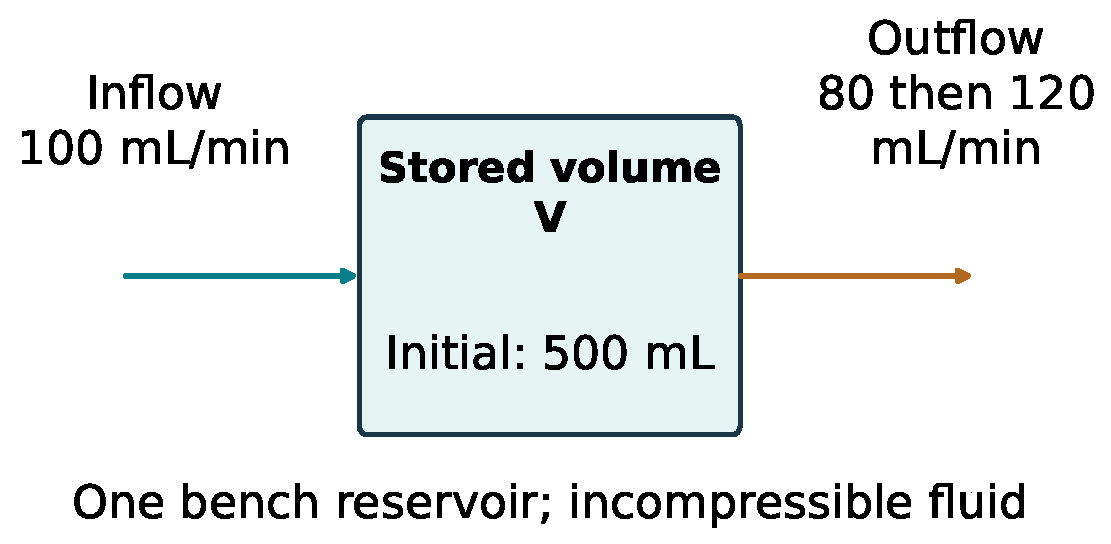
\includegraphics[width=.98\linewidth,height=.69\textheight,keepaspectratio]{presentation-figures/reservoir.pdf}\end{frame}
\renewcommand{\notestarget}{notes.pdf\#note-a-circulation-diagram-determines-an-accounting-boundary}
\begin{frame}[t,fragile,label=slide-the-reservoir-boundary]{The reservoir boundary}
Assume incompressible fluid and no unrecorded transfer. The arrows prescribe rates.\pause{}\[ [V]=\mathrm{mL},\qquad [Q]=\mathrm{mL}/\mathrm{min}.\]What additional relation would be needed to calculate the flows themselves?
\end{frame}
\renewcommand{\notestarget}{notes.pdf\#note-from-transferred-amounts-to-an-integral-balance}
\begin{frame}[t,fragile,label=slide-add-small-transferred-amounts]{Add small transferred amounts}
On a short piece, $\Delta A_{\rm in}\approx Q_{\rm in}(t_k)\Delta t_k$.\pause{}\[A_{\rm in}(t_0,t_1)=\lim\sum_k Q_{\rm in}(t_k)\Delta t_k=\int_{t_0}^{t_1}Q_{\rm in}(s)\,ds.\]The integral adds volume, not flow.
\end{frame}
\renewcommand{\notestarget}{notes.pdf\#note-from-transferred-amounts-to-an-integral-balance}
\begin{frame}[t,fragile,label=slide-conservation-before-differentiation]{Conservation before differentiation}
\[\boxed{V(t_1)-V(t_0)=\int_{t_0}^{t_1}(Q_{\rm in}-Q_{\rm out})\,ds.}\]\pause{}\[V(t_0)=V_0\]An initial value fixes which member of the solution family describes the experiment.
\end{frame}
\renewcommand{\notestarget}{notes.pdf\#note-from-transferred-amounts-to-an-integral-balance}
\begin{frame}[t,fragile,label=slide-the-local-equation]{The local equation}
\[\frac{V(t+h)-V(t)}h=\frac1h\int_t^{t+h}(Q_{\rm in}-Q_{\rm out})\,ds.\]\pause{} At a continuity point of the input, let $h\to0$:\[\boxed{\dot V=Q_{\rm in}-Q_{\rm out}.}\]
\end{frame}
\renewcommand{\notestarget}{notes.pdf\#note-from-transferred-amounts-to-an-integral-balance}
\begin{frame}[t,fragile,label=slide-unit-conversion-is-part-of-the-calculation]{Unit conversion is part of the calculation}
\[(100\ \mathrm{mL}/\mathrm{min})(30\ \mathrm{s})\frac{1\ \mathrm{min}}{60\ \mathrm{s}}=50\ \mathrm{mL}.\]\pause{} A volume divided by a flow has units of time, but its interpretation still depends on the flow law.
\end{frame}
\renewcommand{\notestarget}{notes.pdf\#note-an-exact-switched-flow-experiment}
\begin{frame}[t,fragile,label=slide-first-constant-flow-interval]{First constant-flow interval}
\[V_0=500,\quad Q_{\rm in}=100,\quad Q_{\rm out}=80.\]\pause{}\[V(t)=500+(100-80)t,\qquad V(3)=560\ \mathrm{mL}.\]Entry is $300$ mL; storage gain is only $60$ mL.
\end{frame}
\renewcommand{\notestarget}{notes.pdf\#note-an-exact-switched-flow-experiment}
\begin{frame}[t,fragile,label=slide-switch-the-rate-preserve-the-state]{Switch the rate, preserve the state}
At $t=3$, change the outflow to $120\ \mathrm{mL}/\mathrm{min}$.\pause{}\[V(t)=560-20(t-3),\qquad3\leq t\leq6.\]\[V(3^-)=V(3^+)=560,\qquad V(6)=500.\]
\end{frame}
\renewcommand{\notestarget}{notes.pdf\#note-an-exact-switched-flow-experiment}
\begin{frame}[label=slide-piecewise-linear-storage-panel-1]{Prescribed inflow and outflow}
\centering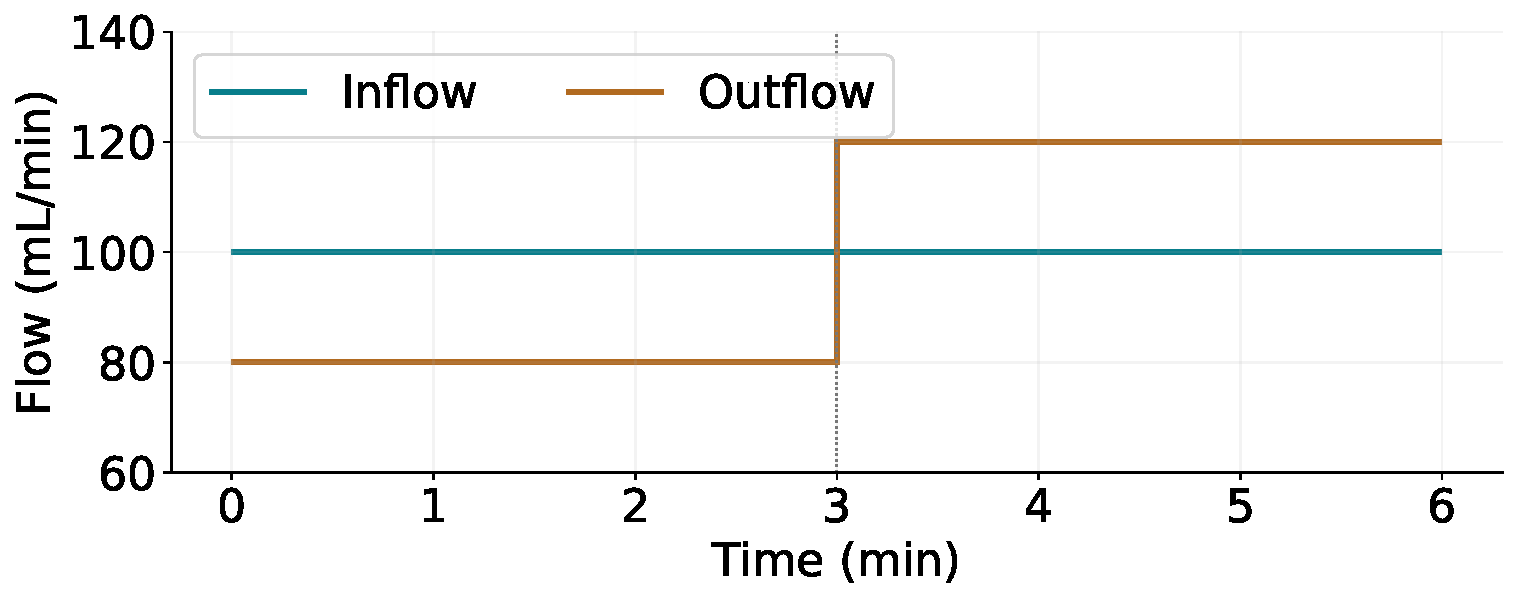
\includegraphics[width=.98\linewidth,height=.69\textheight,keepaspectratio]{presentation-figures/flow-input-panel.pdf}\end{frame}
\renewcommand{\notestarget}{notes.pdf\#note-an-exact-switched-flow-experiment}
\begin{frame}[label=slide-piecewise-linear-storage-panel-2]{The resulting stored volume}
\centering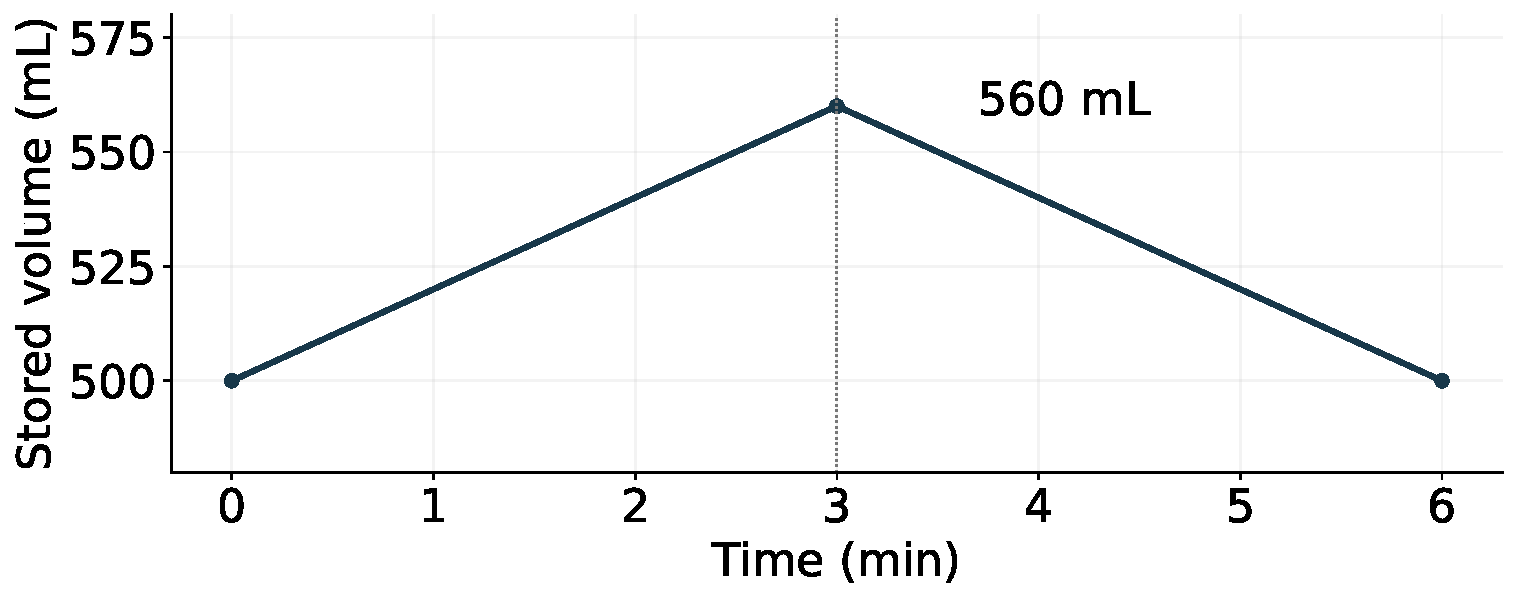
\includegraphics[width=.98\linewidth,height=.69\textheight,keepaspectratio]{presentation-figures/volume-storage-panel.pdf}\end{frame}
\renewcommand{\notestarget}{notes.pdf\#note-an-exact-switched-flow-experiment}
\begin{frame}[t,fragile,label=slide-piecewise-linear-storage]{Piecewise-linear storage}
\[\dot V=+20\quad(t<3),\qquad \dot V=-20\quad(t>3).\]\pause{} A finite rate jump changes slope. A finite volume jump would require an impulsive transfer.
\end{frame}
\renewcommand{\notestarget}{notes.pdf\#note-an-exact-switched-flow-experiment}
\begin{frame}[t,fragile,label=slide-check-the-entire-experiment]{Check the entire experiment}
\[A_{\rm in}=100(6)=600,\qquad A_{\rm out}=80(3)+120(3)=600.\]\pause{}\[V_0+A_{\rm in}=V(6)+A_{\rm out}.\]The endpoint returns to its initial value despite nonzero throughput.
\end{frame}
\renewcommand{\notestarget}{notes.pdf\#note-an-exact-switched-flow-experiment}
\begin{frame}[t,fragile,label=slide-steady-storage-permits-throughput]{Steady storage permits throughput}
\[\dot V=0\quad\Longleftrightarrow\quad Q_{\rm in}=Q_{\rm out}.\]\pause{} Both $(Q_{\rm in},Q_{\rm out})=(0,0)$ and $(100,100)$ satisfy it. Volume alone cannot identify replacement or mixing.
\end{frame}
\renewcommand{\notestarget}{notes.pdf\#note-why-internal-transfers-disappear-from-a-larger-balance}
\begin{frame}[t,fragile,label=slide-enlarge-the-boundary]{Enlarge the boundary}
\[\dot V_1=a-q,\qquad\dot V_2=q-b.\]\pause{}\[\boxed{\frac{d}{dt}(V_1+V_2)=a-b.}\]The same internal transfer must appear with opposite signs.
\end{frame}
\renewcommand{\notestarget}{notes.pdf\#note-why-internal-transfers-disappear-from-a-larger-balance}
\begin{frame}[t,fragile,label=slide-the-network-version-of-the-same-argument]{The network version of the same argument}
An incidence column has one $-1$ and one $+1$.\[\dot{\mathbf V}=B\mathbf Q+\mathbf u.\]\pause{}\[\mathbf1^TB=0\quad\Rightarrow\quad\frac{d}{dt}\sum_iV_i=\sum_i u_i.\]
\end{frame}
\renewcommand{\notestarget}{notes.pdf\#note-admissibility-and-the-emptying-event}
\begin{frame}[t,fragile,label=slide-locate-the-first-impossible-continuation]{Locate the first impossible continuation}
If $r=Q_{\rm in}-Q_{\rm out}<0$,\[V(t_k+s)=V_k+rs.\]\pause{}\[\tau=V_k/(-r),\qquad50/20=2.5\ \mathrm{min}.\]Stop or change the model at emptying; clipping hides a transfer.
\end{frame}
\renewcommand{\notestarget}{notes.pdf\#note-exact-interval-updates-and-evidence-for-the-model}
\begin{frame}[t,fragile,label=slide-an-exact-interval-algorithm]{An exact interval algorithm}
For each constant-rate interval:\[\Delta V_k=(Q_{{\rm in},k}-Q_{{\rm out},k})\Delta t_k,\quad V_{k+1}=V_k+\Delta V_k.\]\pause{} Reject an inadmissible interval. Splitting an interval into two pieces must give the same endpoint.
\end{frame}
\renewcommand{\notestarget}{notes.pdf\#note-exact-interval-updates-and-evidence-for-the-model}
\begin{frame}[t,fragile,label=slide-a-residual-checks-the-account]{A residual checks the account}
\[\mathcal R_k=V_k-V_0-\sum_{j<k}(Q_{{\rm in},j}-Q_{{\rm out},j})\Delta t_j.\]\pause{} $\mathcal R_k\approx0$ checks implementation. It cannot reveal an omitted leak that is absent from both code and equations.
\end{frame}
\renewcommand{\notestarget}{notes.pdf\#note-exact-interval-updates-and-evidence-for-the-model}
\begin{frame}[t,fragile,label=slide-model-discrepancy]{Model discrepancy}
Predict $V(t)$ using independently measured flows.\pause{}\[e(t)=V^{\rm obs}(t)-V^{\rm pred}(t).\]Inspect the time pattern, the measurement uncertainty, and the first violated assumption.
\end{frame}
\end{document}
